\section{Digitala kretsar}
\index{digitala kretsar}
\label{digitala kretsar}

Särskilt under det senaste decenniet har digital elektronik blivit vanlig i
utrustningar för radio- och telekommunikation. Även inom amatörradio används nu
denna teknik. Ämnet är mycket omfattande. Utvecklingen är att enkla digitala
funktioner snabbt ersätts av komplexa datasystem. Här redogörs endast för några
grundläggande digitala funktioner.

Amatörradions kärna finns ännu i \emph{analogtekniken}, där det under ett
förlopp kan förekomma många olika storheter, t.ex. spänningar mellan noll och
ett högsta värde.

I digitaltekniken förekommer bara ett bestämt antal tillstånd. I det enklaste
digitala systemet finns två tillstånd, t.ex. 0 och 1 eller Till och Från eller
Hög och Låg eller Fel och Rätt o.s.v. Ett system med två tillstånd kallas
binärt. En lampa som tänds eller släcks med en enkel strömställare är ett binärt
system. Strömställaren kan ha olika utföranden. Det kan vara en mekanisk kontakt
som är styrd för hand eller av en reläspole. Det kan också vara en transistor
eller annan anordning.

\subsection{Transistorn som strömställare}

\begin{figure}
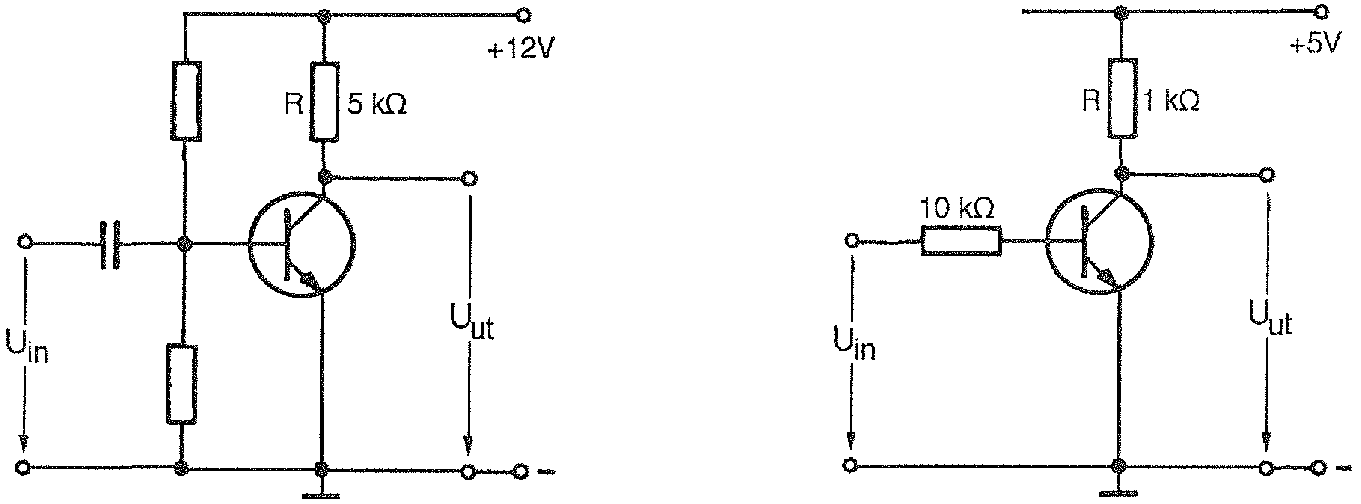
\includegraphics[width=\textwidth]{images/bild_2_2-35}
\caption{Transistorn som analog förstärkare respektive digital strömställare}
\label{fig:BildII2-35}
\end{figure}

Bild \ref{fig:BildII2-35}

Bilden visar två transistorkopplingar. Den till vänster är en analog förstärkare
för växelspänning. Om det på grund av en viss basspänning flyter en
kollektorström av 1~mA och kollektorresistorn är 5~Ω, så blir spänningsfallet
över den resistorn 5~V. Eftersom matningsspänningen är 12~V, så blir då
spänningen 7~V mellan kollektorn och minus.

Kopplingen till höger fungerar som en binär strömställare. Antag att insignalen
intar ett avtvå spänningstillstånd, antingen 0 V (låg) eller SV (hög). När
inspänningen är t.ex. 5~V, så flyter så mycket basström genom basresistorns
1O~kΩ, att transistorn blir fullt utstyrd.

Därmed är spänningen mellan kollektor och emitter, d.v.s. utspänningen, nära 0~V
(0.1 till 0.2~V beroende på transistortyp). Man säger då att utgången är låg (L)
eller 0 (noll).

Om däremot inspänningen är 0~V, sås pärras kollektorströmmen och utspänningen
blir nära 5~V. Man säger då att utgången är hög (H) eller 1.

För NPN-transistorn i bilden, gäller att
\begin{itemize}
\item hög inspänning ger låg utspänning,
\item låg inspänning ger hög utspänning.
\end{itemize}
Denna logiska funktion kallas inverterande.

\subsubsection{NOT-gate eller inverterande grind}
\index{inverterande grind}
\index{NOT-gate}

\begin{wrapfigure}[6]{R}{0.5\textwidth}
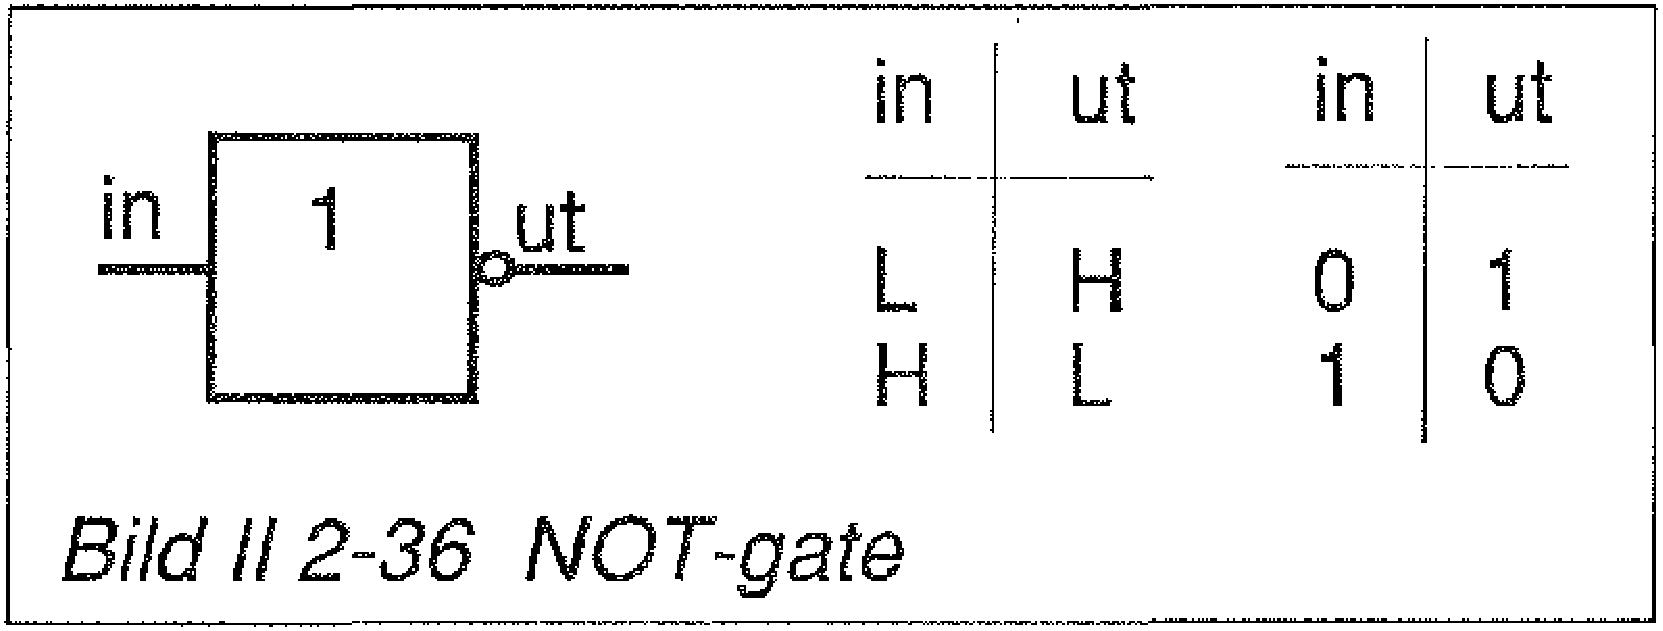
\includegraphics[width=0.5\textwidth]{images/bild_2_2-36}
\caption{NOT-gate}
\label{fig:BildII2-36}
\end{wrapfigure}

Bild \ref{fig:BildII2-36}

Logiska funktioner beskrivs med internationella symboler. En ring vid utgången
betyder att utspänningens nivå är motsatt inspänningens. Sambandet mellan in-
och utnivåerna beskrivs med en \emph{sanningstabell}.

\subsection{Villkorskretsar - s.k. grindar}

Det finns olika sätt att bygga grindar. Idag är de flesta grindarna elektroniska
lösningar. Därutöver finns elektromekaniska grindar i form av strömbrytare och
reläkontakter.

Föregångarna till de elektroniska televäxlarna (AXE m.fl.) var stora system av
mestadels elektromekaniska reläer.

För att överskådligt förklara arbetssättet i de vanligaste grindarna, görs det
enklast med reläsymboler. En reläkontakt kan då motsvara en transistor eller
diod. Reläspolar kan motsvara logiska nivåer i insignaler.

Elektriska kontakter kan vara normalt öppna och sluter vid påverkan (s.k.
slutande kontakt). Alternativt kan de vara normalt slutna och öppnar vid
påverkan (s.k. brytande kontakt). I kretsscheman visas kontaktlägena vid
systemet i vila.

Av bilden framgår att samma villkor kan skapas med slutande alternativt brytande
kontakter. Observera då placeringen av resistorn på kretsens utgångssida i
respektive fall. När resistorn ligger närmast pluspolen kallas den pull-up. När
den ligger närmast minuspolen kallas den pull-down. I båda fallen definierar
resistorn den logiska nivån.

\subsubsection{OCH-grind eller AND-gate}
\index{AND-gate}

\begin{figure}
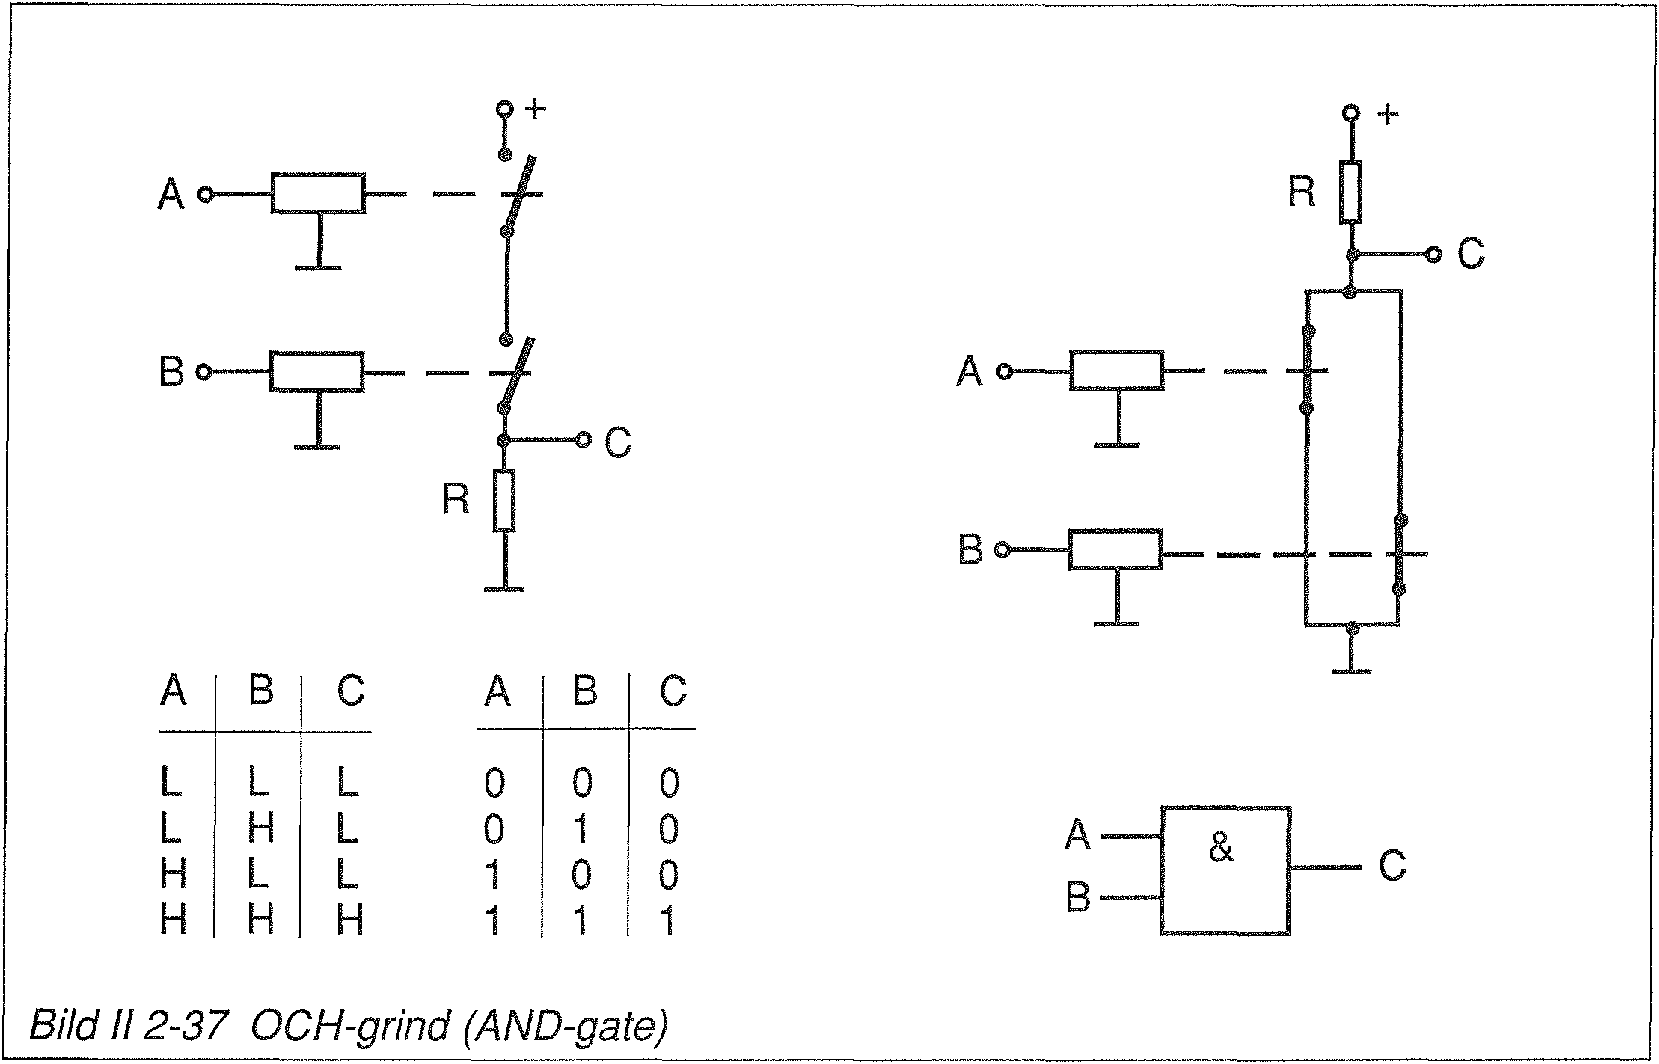
\includegraphics[width=\textwidth]{images/bild_2_2-37}
\caption{OCH-grind (AND-gate)}
\label{fig:BildII2-37}
\end{figure}

Bild \ref{fig:BildII2-37}

Sanningstabellen i bilden säger, att när alla insignaler är 1 så är utsignalen
också 1.

\subsubsection{ELLER-grind eller OR-gate}
\index{OR-gate}

\begin{figure}
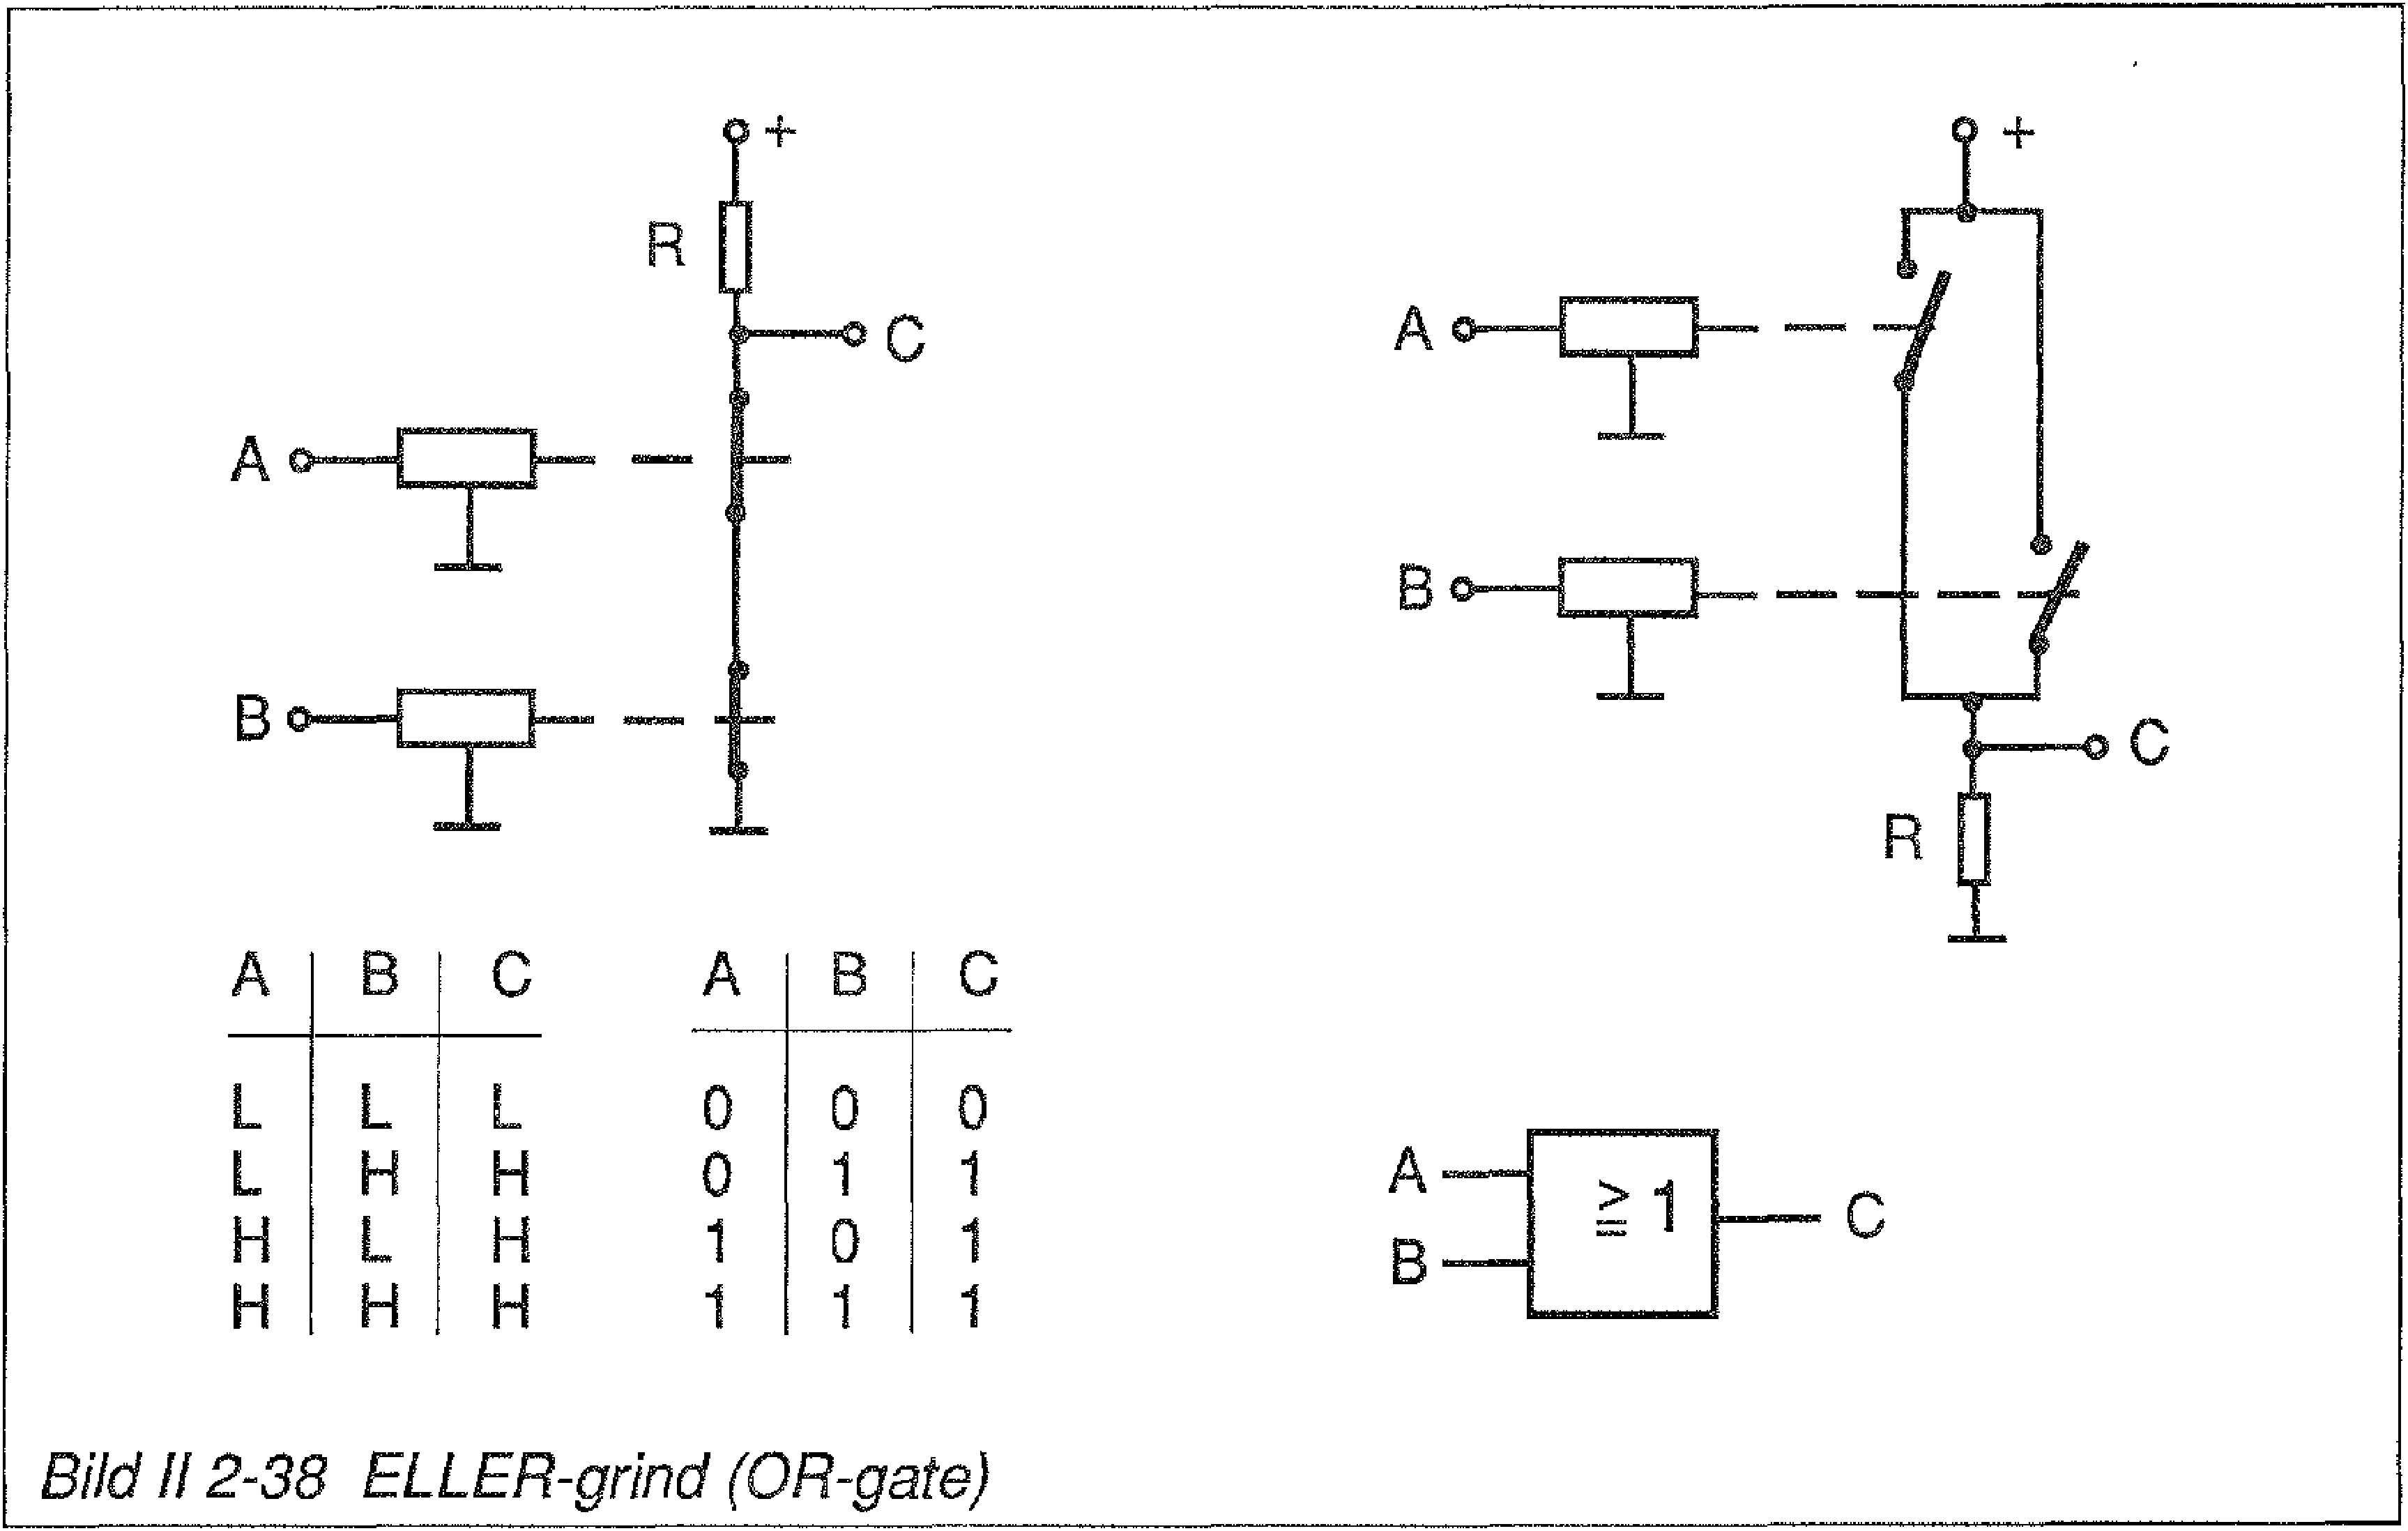
\includegraphics[width=\textwidth]{images/bild_2_2-38}
\caption{ELLER-grind (OR-gate)}
\label{fig:BildII2-38}
\end{figure}

Bild \ref{fig:BildII2-38}

Sanningstabellen säger, att när en eller flera av insignalerna är 1 så är
utsignalen också 1. När alla insignaler är 0, så är utsignalen 0.

\subsubsection{OCH INTE-grind eller NAND-gate}
\index{NAND-gate}

\begin{figure}
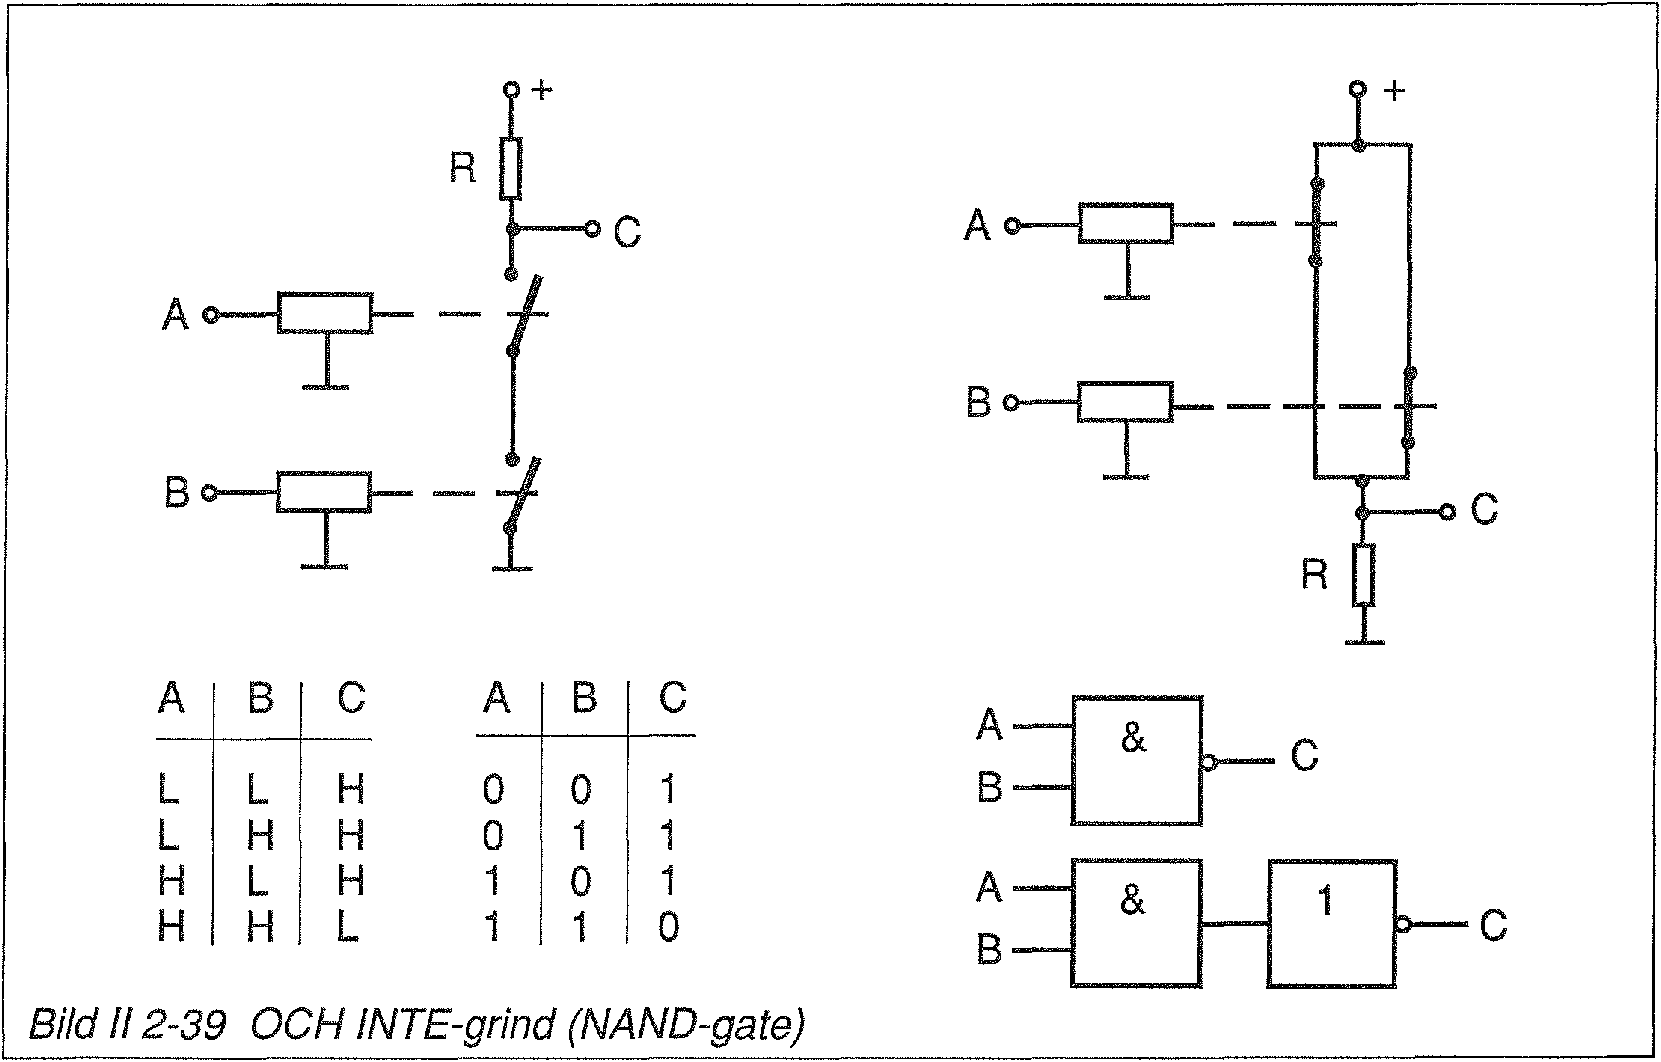
\includegraphics[width=\textwidth]{images/bild_2_2-39}
\caption{OCH INTE-grind (NAND-gate)}
\label{fig:BildII2-39}
\end{figure}

Bild \ref{fig:BildII2-39}

Sanningstabellen säger, att när ingen eller någon insignal är 1, men inte alla,
så är utsignalen 1. När alla insignaler är 1, så är utsignalen 0.

\subsubsection{INTE ELLER-grind eller NOR-gate}
\index{NOR-gate}

\begin{figure}
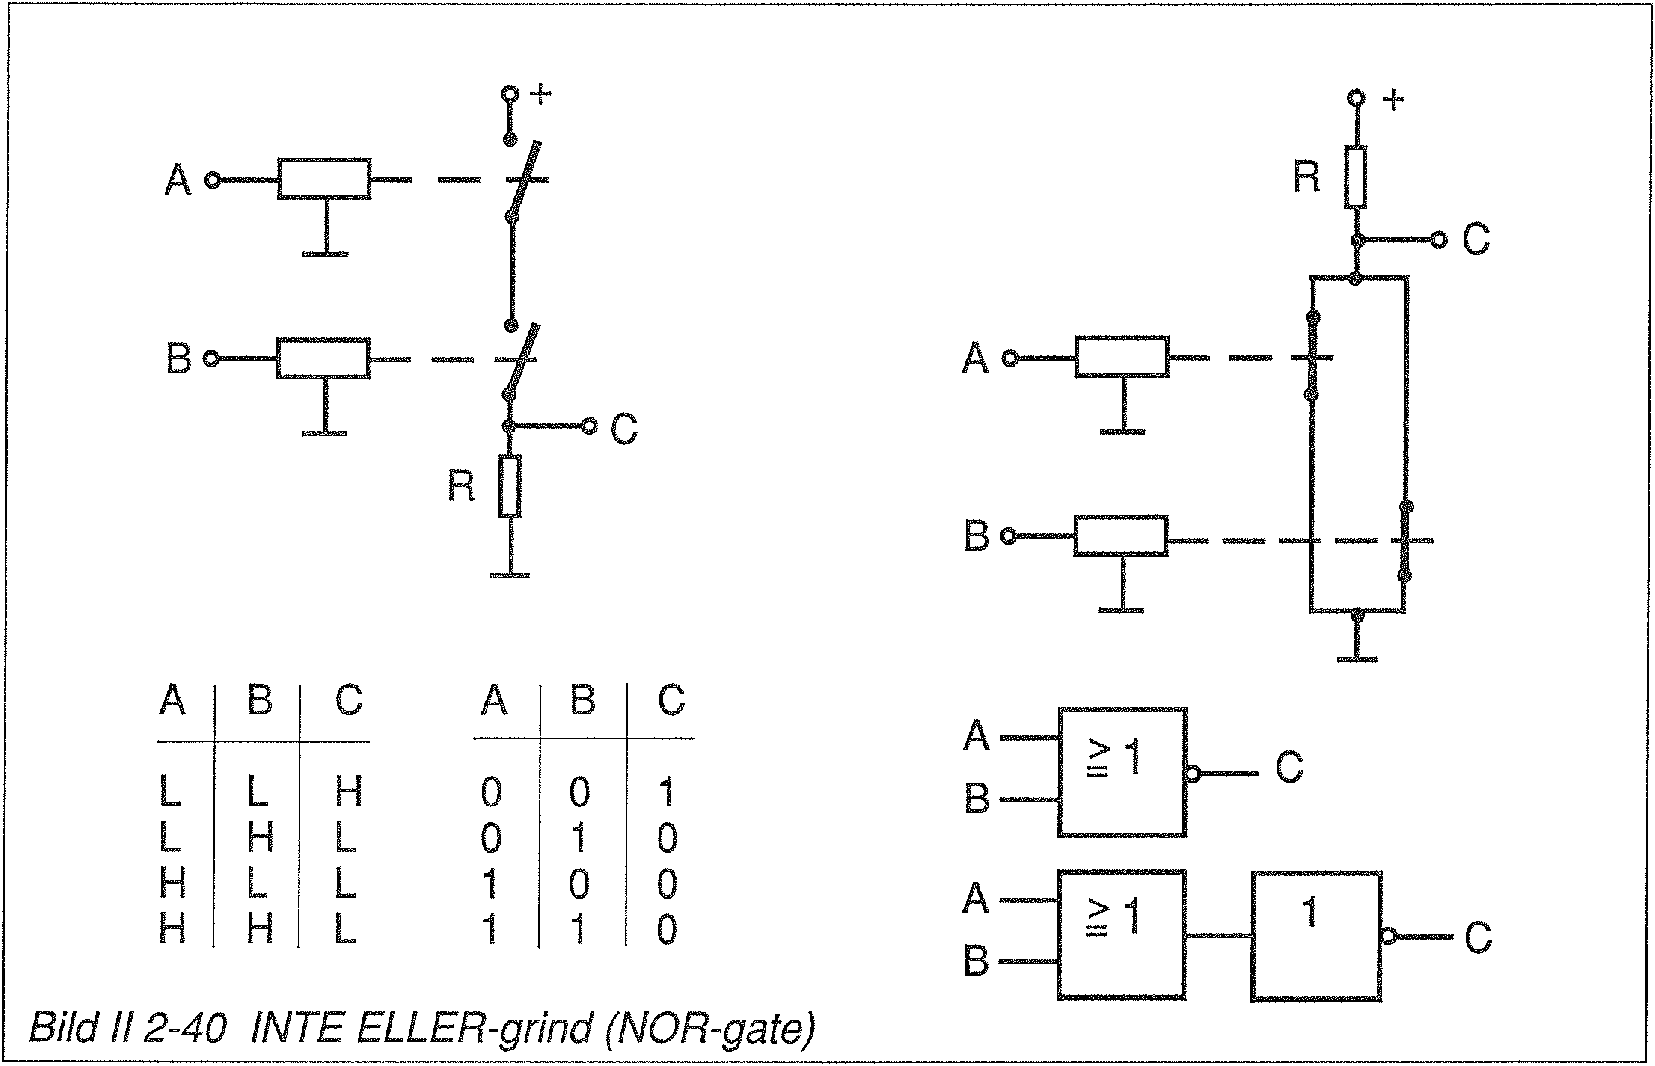
\includegraphics[width=\textwidth]{images/bild_2_2-40}
\caption{INTE ELLER-grind (NOR-gate)}
\label{fig:BildII2-40}
\end{figure}

Bild \ref{fig:BildII2-40}

Sanningstabellen säger, att när någon eller alla insignaler är 1, så är
utsignalen 0. När alla insignaler är 0, så är utsignalen 1.

\subsubsection{Inverterad ingång}

En ingång kan behöva ha en inverterad funktion i förhållande till de övriga
(s.k. low active). Man kan då göra på följande sätt med en OCH-grind som
exempel.

\begin{wrapfigure}{R}{0.5\textwidth}
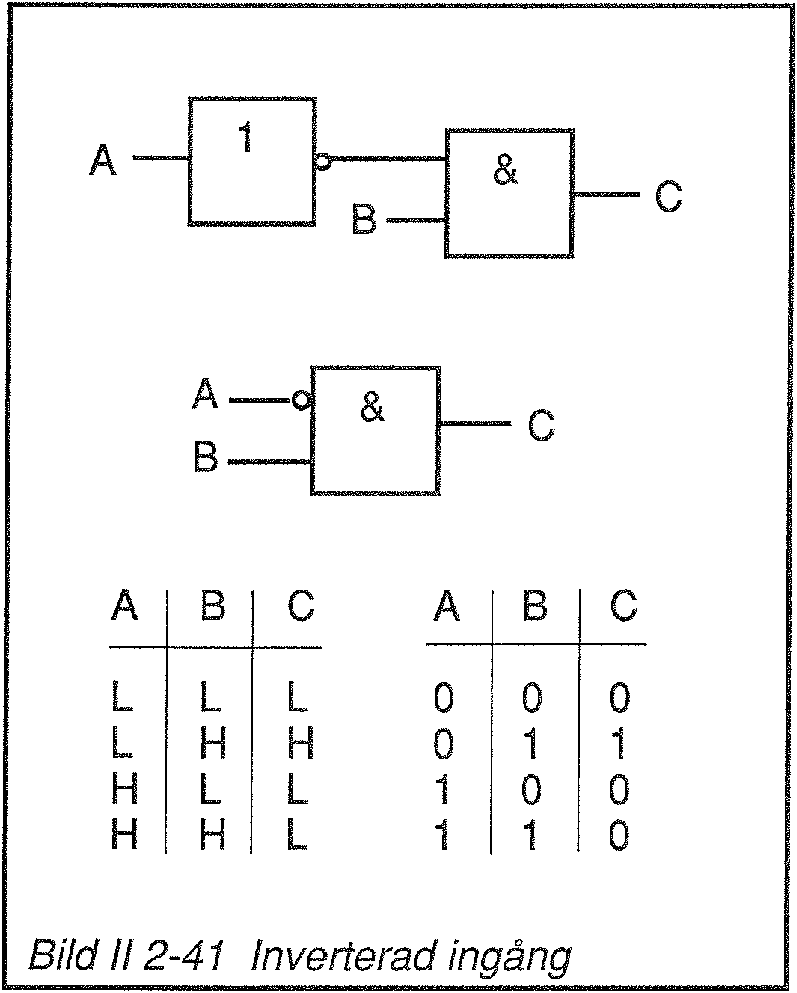
\includegraphics[width=0.5\textwidth]{images/bild_2_2-41}
\caption{Inverterad ingång}
\label{fig:BildII2-41}
\end{wrapfigure}

Bild \ref{fig:BildII2-41}

\subsubsection{Exklusiv ELLER-grind (XOR-gate)}
\index{XOR-gate}

\begin{wrapfigure}{R}{0.5\textwidth}
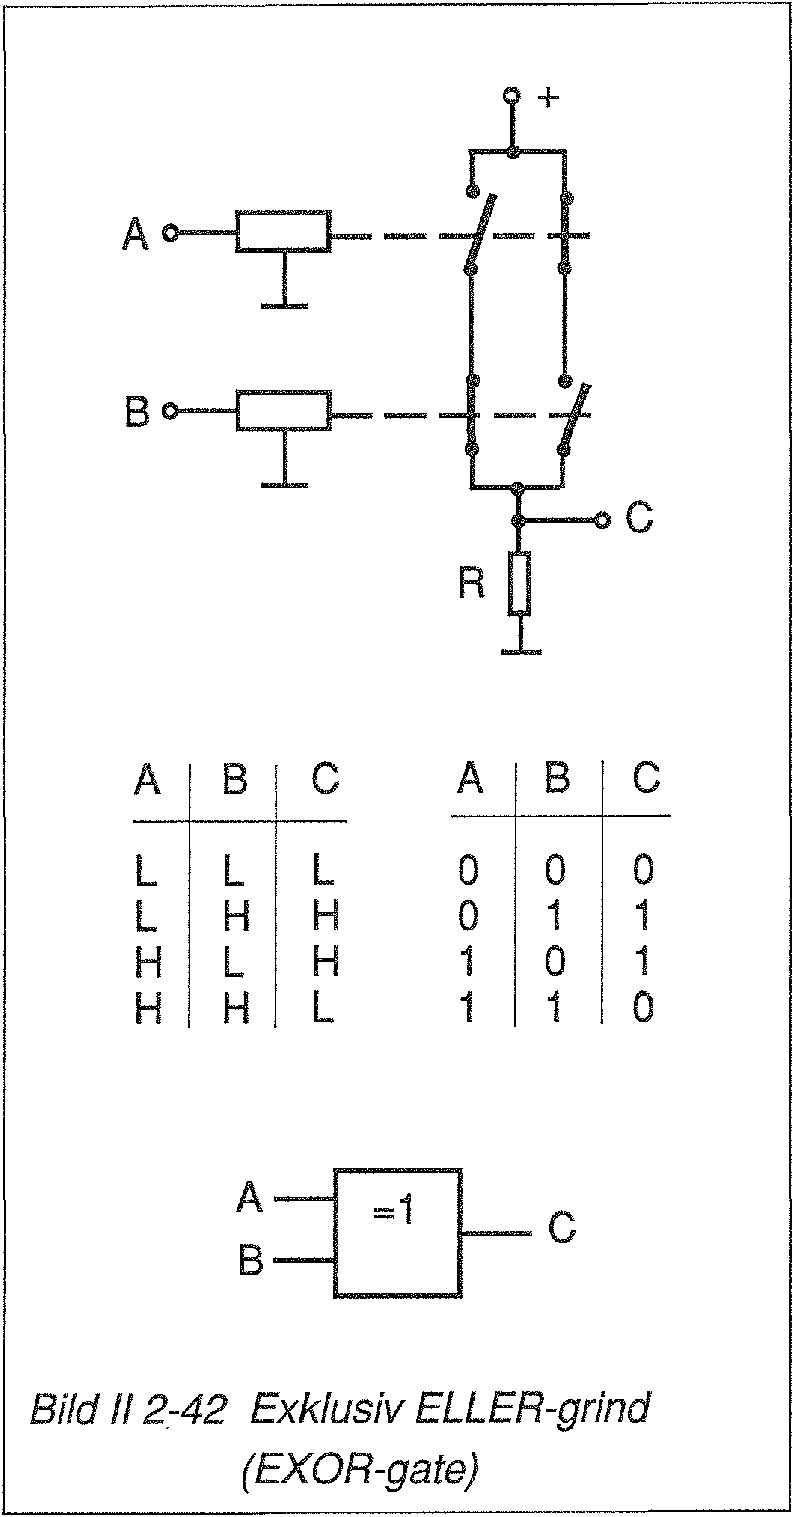
\includegraphics[width=0.5\textwidth]{images/bild_2_2-42}
\caption{Exklusiv ELLER-grind (EXOR-gate)}
\label{fig:BildII2-42}
\end{wrapfigure}

Bild \ref{fig:BildII2-42}

Sanningstabellen säger, att när alla insignaler antingen är 1 eller 0, så är
utsignalen 0. När en, men inte alla insignaler är i, så är utsignalen 1.

\subsubsection{Exklusiv INTE ELLER-grind (XNOR-gate)}
\index{XNOR-gate}

\begin{wrapfigure}{R}{0.5\textwidth}
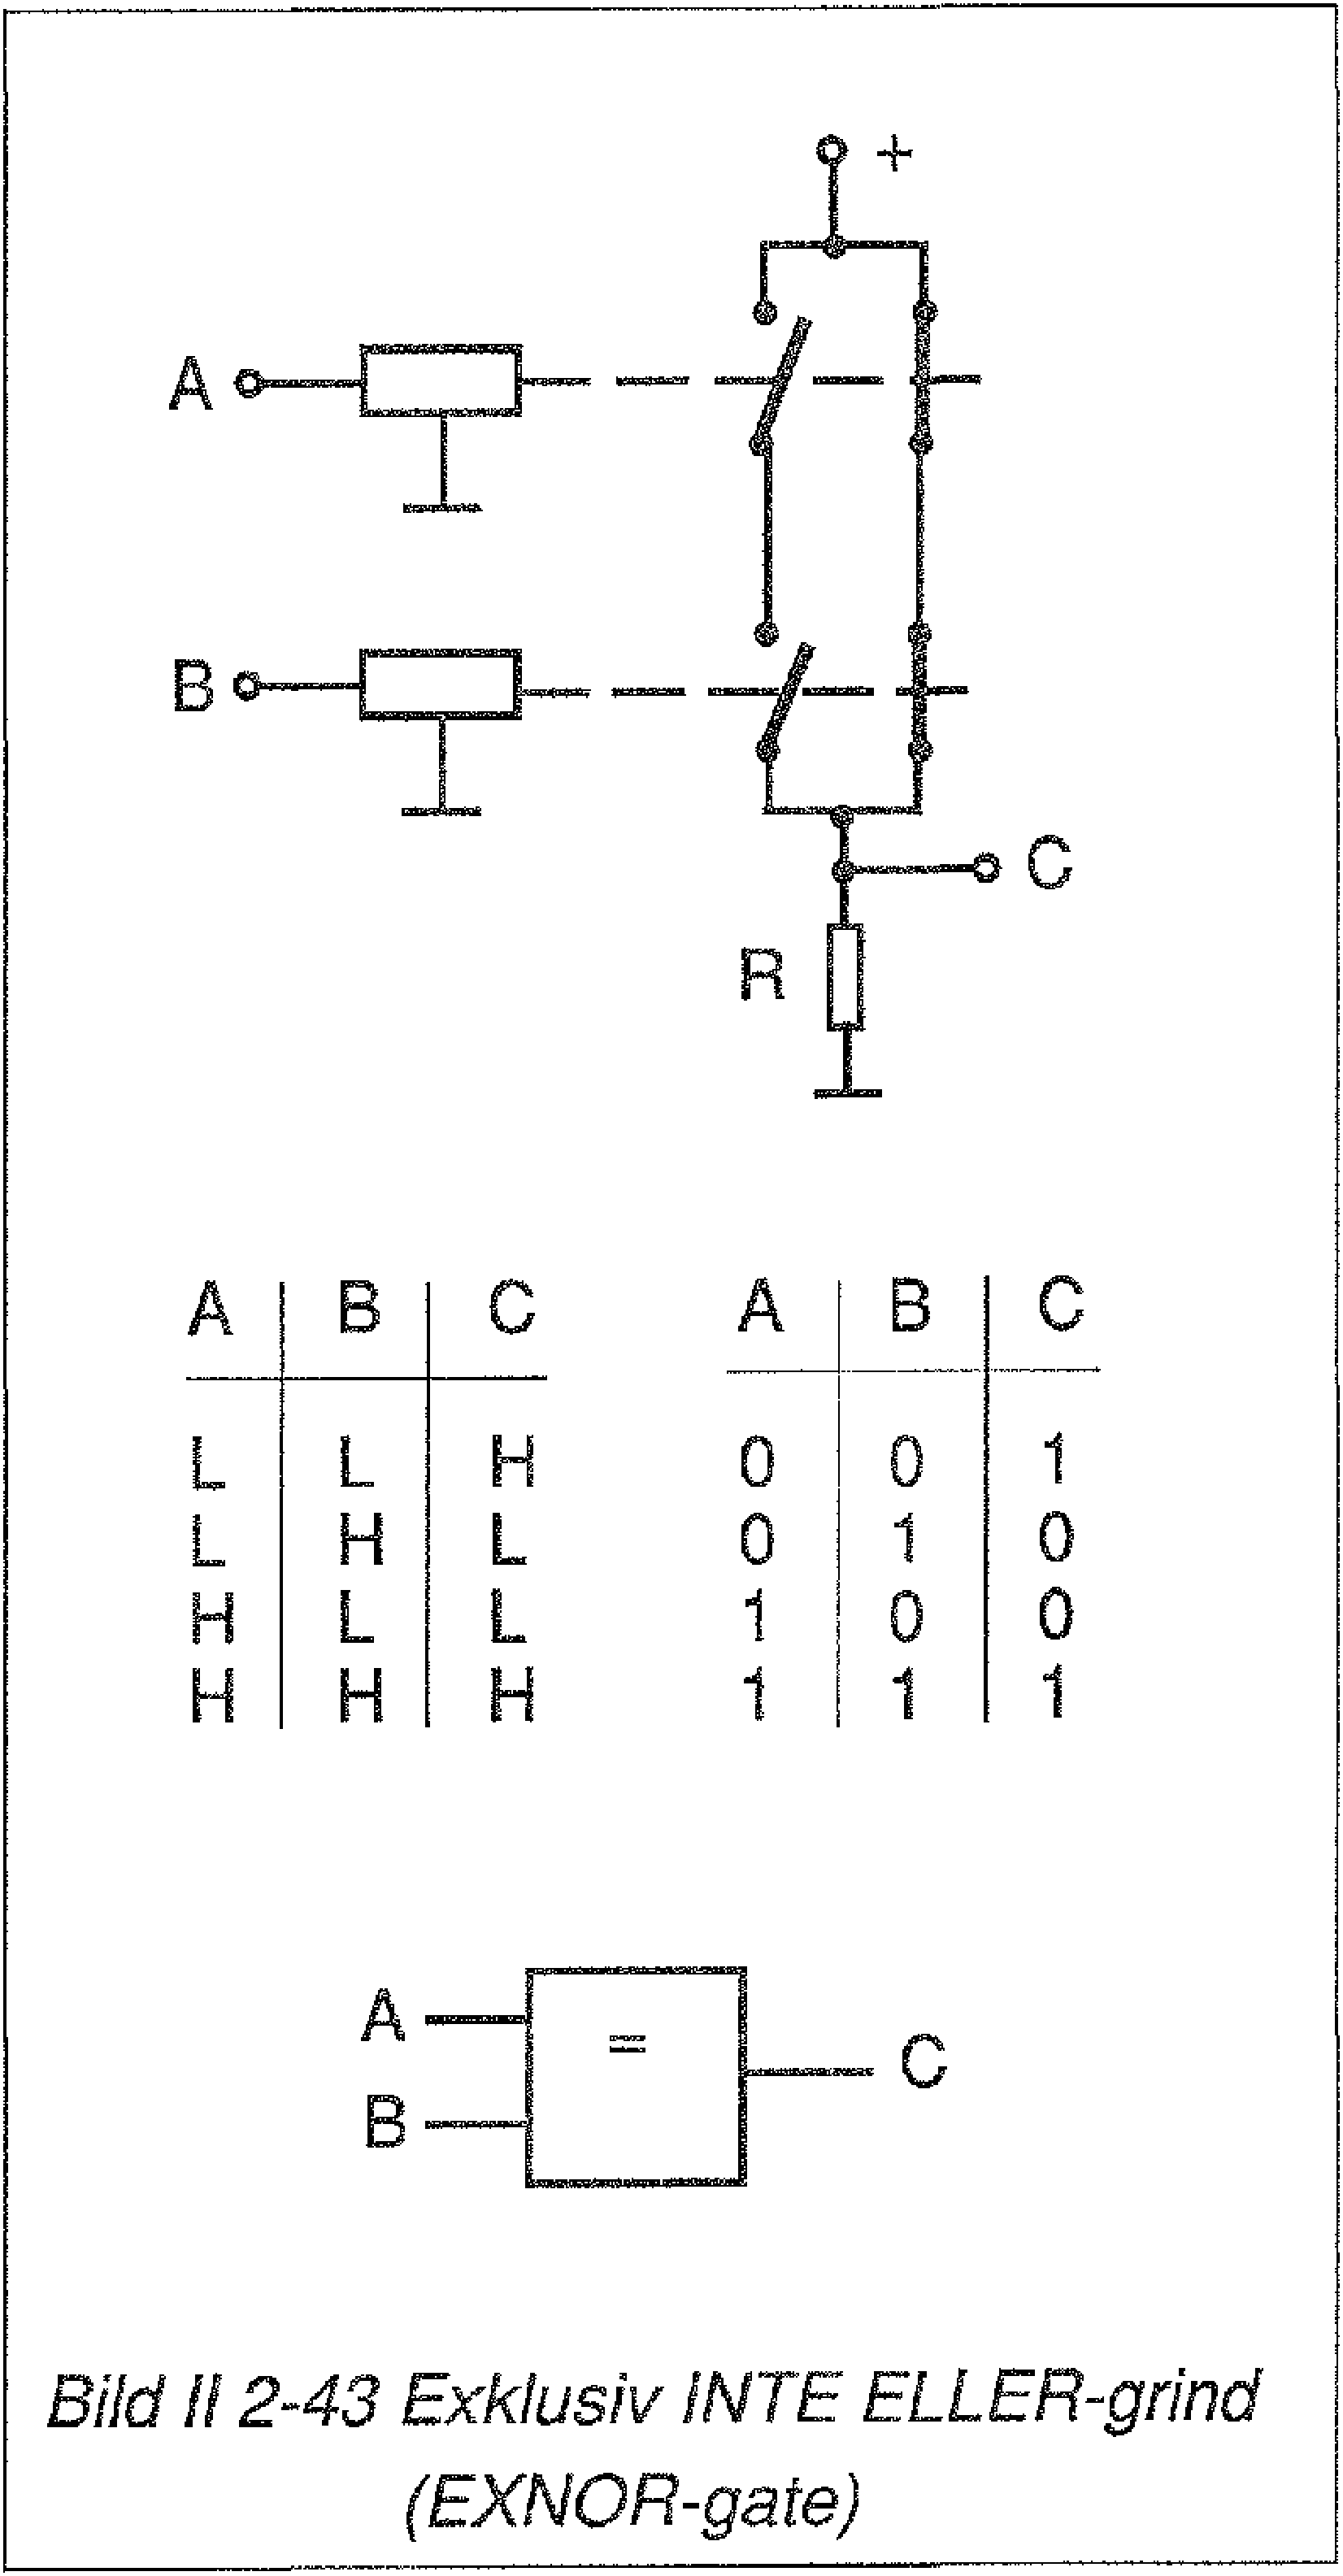
\includegraphics[width=0.5\textwidth]{images/bild_2_2-43}
\caption{Exklusiv INTE ELLER-grind (EXNOR-gate)}
\label{fig:BildII2-43}
\end{wrapfigure}

Bild \ref{fig:BildII2-43}

Sanningstabellen säger, att när alla insignaler antingen är 1 eller 0, så är
utsignalen 1. När en, men inte alla insignaler är 1, så är utsignalen 0.

\subsection{Grindar med dioder och transistorer}

I stället för reläer i grindar använder man nu ytterst sällan något annat än
kombinationer av dioder, transistorer och resistorer.

\begin{wrapfigure}{R}{0.5\textwidth}
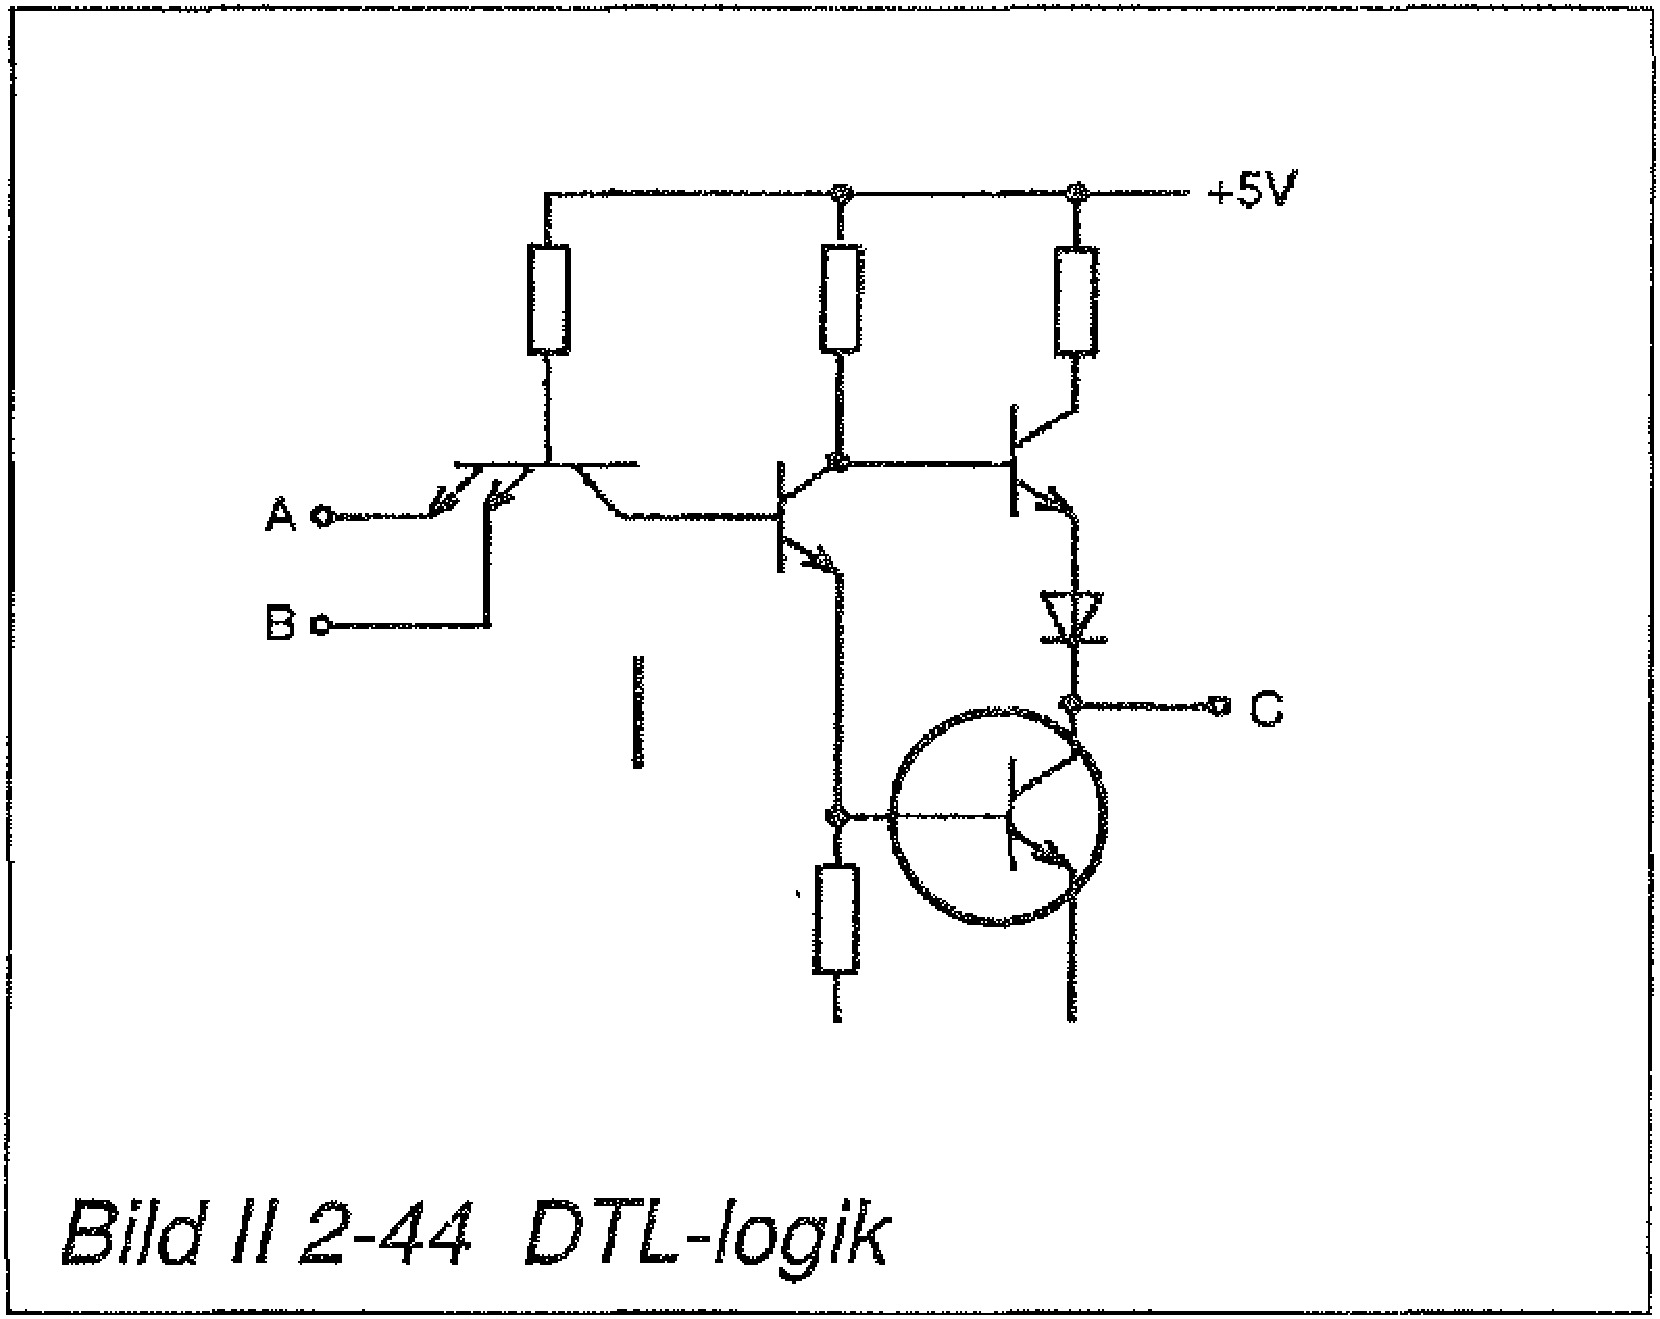
\includegraphics[width=0.5\textwidth]{images/bild_2_2-44}
\caption{DTL-logik}
\label{fig:BildII2-44}
\end{wrapfigure}

Bild \ref{fig:BildII2-44}

Bilden visar en NAND-grind. Den egentliga grinden består av tre dioder och en
resistor. Två av dioderna är ingångar och den tredje är utgång. Grinden styr en
digitalt arbetande transistor liksom den i bild \ref{fig:BildII2-35}.
Resultatet är en s.k. DTL-logik.

\begin{wrapfigure}{R}{0.5\textwidth}
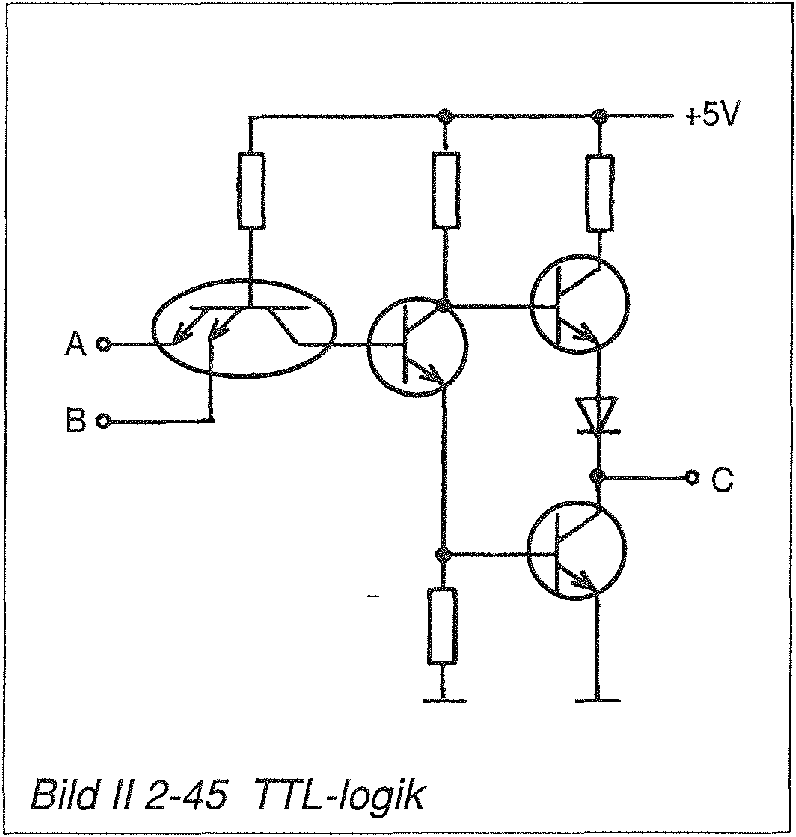
\includegraphics[width=0.5\textwidth]{images/bild_2_2-45}
\caption{TTL-logik}
\label{fig:BildII2-45}
\end{wrapfigure}

Bild \ref{fig:BildII2-45}

Även denna bild visar en NAND-grind. Här består den egentliga grinden av en
ingångstransistor med två emittrar, vilka motsvarar dioderna vid A och B i
föregående bild. Kollektorn i denna transistor motsvarar ingångsdioden till
transistorn i bild \ref{fig:BildII2-44}. De övriga tre transisitorerna i bild
\ref{fig:BildII2-45} bildar en s.k. switch, som ger snabb övergång mellan väl
definierade logiska nivåer. Resultatet är en s.k. TTL-logik.
